% ============================================================
%  best_equipo_03.tex: deck del mejor modelo.
%  Se compila con XeLaTeX desde 04_slides/compile_slides.R. Las figuras,
%  tablas y cifras no se copian aquí: se leen de 02_outputs/, donde las
%  escriben los scripts 16 y 17 de 01_code/, para que el PDF siempre
%  muestre los resultados de la última corrida.
% ============================================================
\documentclass[aspectratio=169, 10pt]{beamer}

% ---------- Tema ----------
\usetheme{metropolis}

% ---------- Idioma y codificación ----------
\usepackage[utf8]{inputenc}
\usepackage[spanish,provide=*]{babel}
\usepackage[T1]{fontenc}

% ---------- Fuente: Calibri (vía Carlito, su equivalente libre) ----------
\usepackage{ifxetex,ifluatex}
\newif\ifxetexorluatex
\ifxetex\xetexorluatextrue\fi
\ifluatex\xetexorluatextrue\fi
\ifxetexorluatex
  \usepackage{fontspec}
  % Se carga por nombre de archivo para que XeLaTeX la encuentre tanto en
  % las fuentes del sistema como en la distribución de LaTeX (TinyTeX).
  \setmainfont{Carlito}[Extension = .ttf, UprightFont = *-Regular,
    BoldFont = *-Bold, ItalicFont = *-Italic, BoldItalicFont = *-BoldItalic]
  \setsansfont{Carlito}[Extension = .ttf, UprightFont = *-Regular,
    BoldFont = *-Bold, ItalicFont = *-Italic, BoldItalicFont = *-BoldItalic]
\else
  \PackageWarningNoLine{plantilla}{Compila con XeLaTeX o LuaLaTeX para usar la fuente Calibri/Carlito}
\fi

% ---------- Matemáticas ----------
\usepackage{amsmath, amssymb}

% ---------- Gráficos, tablas y código ----------
\usepackage{graphicx}
\graphicspath{{../02_outputs/figures/}}
\usepackage{tikz}
\usetikzlibrary{positioning, arrows.meta, shapes.geometric, calc, fit, backgrounds}
\usepackage{booktabs}
\usepackage{array}
\usepackage{changepage}

% ---------- Paleta de acento ----------
\definecolor{accent}{HTML}{2E5EAA}
\definecolor{azuloscuro}{HTML}{0F3570}
\definecolor{azulclaro}{HTML}{9CC3EE}
\setbeamercolor{palette primary}{bg=accent, fg=white}
\setbeamercolor{progress bar}{fg=accent, bg=accent!20}
\setbeamercolor{frametitle}{bg=accent}
\setbeamercolor{alerted text}{fg=accent}

% ---------- Ajustes de Metropolis ----------
\setbeamertemplate{section in toc}[sections numbered]
\setbeamertemplate{frame numbering}[fraction]
\metroset{block=fill, sectionpage=none, numbering=fraction, progressbar=none}

% ---------- Ajustes propios ----------
% Cajas (block) con margen interno, para que el texto no toque los bordes.
\setbeamertemplate{block begin}{%
  \par\vskip\medskipamount%
  \begin{beamercolorbox}[colsep*=.5ex, leftskip=0.4ex, sep=0.9ex, vmode]{block title}%
    \usebeamerfont*{block title}\insertblocktitle%
  \end{beamercolorbox}%
  \nointerlineskip%
  \begin{beamercolorbox}[colsep*=.5ex, leftskip=0.4ex, sep=1ex, vmode]{block body}%
    \usebeamerfont{block body}%
    \begin{adjustwidth}{0pt}{2.5ex}%
}
\setbeamertemplate{block end}{\end{adjustwidth}\end{beamercolorbox}\vskip\smallskipamount}
% Nota pequeña al pie de una diapositiva (fuente de los datos).
\newcommand{\nota}[1]{\vfill{\scriptsize\color{black!60}#1\par}}
% Las slides después de \appendix no cuentan en la numeración.
\usepackage{appendixnumberbeamer}

% Cifras del mejor modelo (01_code/16_best_model_analysis.R) y del
% análisis de negocio (01_code/17_business_analysis.R).
\newcommand{\MAEKaggle}{164,5}
\newcommand{\MAEBase}{296,6}
\newcommand{\MAELgbm}{178,6}
\newcommand{\MAECVEspacial}{128,6}
\newcommand{\MAECVAleatoria}{94,3}
\newcommand{\MAESimilares}{130,6}
\newcommand{\SesgoSimilares}{-30,5}
\newcommand{\ErrorPct}{23\%}
\newcommand{\PrecioMedioSimilares}{713}
\newcommand{\NTrain}{38.644}
\newcommand{\NTest}{10.286}
\newcommand{\PctSuperficieReal}{56\%}
\newcommand{\PctSuperficieImputada}{44\%}
\newcommand{\NEnsayos}{30}
\newcommand{\TasaAprendizaje}{0,017}
\newcommand{\Hojas}{66}
\newcommand{\Profundidad}{7}
\newcommand{\MinHoja}{23}
\newcommand{\Rondas}{4.123}
\newcommand{\PesoRed}{25\%}
\newcommand{\PesoLgbm}{75\%}
\newcommand{\BrechaElegido}{9,8}
\newcommand{\BrechaCinco}{12,9}
\newcommand{\BrechaAleatoria}{21,3}
\newcommand{\NEsquemas}{8}
\newcommand{\PrometeAleatoria}{21}
\newcommand{\PrometeCinco}{9}
\newcommand{\PrometeVeinte}{3}
\newcommand{\GainUbicacion}{51}
\newcommand{\GainVecinos}{20}
\newcommand{\GainTexto}{25}
\newcommand{\GainVivienda}{22}
\newcommand{\MejoraPctBase}{45\%}
\newcommand{\NRaices}{141}
\newcommand{\MejoraRed}{2,2}
\newcommand{\KaggleAmpliado}{194,4}
\newcommand{\MejoraLMTexto}{81}
\newcommand{\CVEspSinVec}{128,7}
\newcommand{\CVEspConVec}{134,0}
\newcommand{\CVAleSinVec}{97,5}
\newcommand{\CVAleConVec}{95,5}
\newcommand{\KaggleSinVec}{169,2}
\newcommand{\KaggleConVec}{166,7}
\newcommand{\SesgoCaras}{347}
\newcommand{\EjSuperficie}{85}
\newcommand{\EjHabitaciones}{2}
\newcommand{\EjBanos}{2}
\newcommand{\EjEstrato}{4}
\newcommand{\EjVecinosMdos}{5,3}
\newcommand{\EjVecinosDist}{195}
\newcommand{\EjLgbmMdos}{6,4}
\newcommand{\EjLgbm}{548}
\newcommand{\EjRed}{518}
\newcommand{\EjFinal}{540}
\newcommand{\SesgoBaratas}{90}

\newcommand{\PctSobre}{48\%}
\newcommand{\PctSub}{52\%}
\newcommand{\SobrepagoMedio}{104}
\newcommand{\SubestimaMedio}{155}
\newcommand{\FactorKaggle}{1,26}
\newcommand{\MargenCV}{25\%}
\newcommand{\MargenRegla}{30\%}
\newcommand{\RiesgoSinMargen}{48\%}
\newcommand{\RiesgoRegla}{9\%}
\newcommand{\OfertaTipica}{31\%}
\newcommand{\NParecidas}{3.865}
\newcommand{\RiesgoCasa}{28\%}
\newcommand{\RiesgoApto}{8\%}
\newcommand{\RiesgoEstBajo}{15\%}
\newcommand{\RiesgoEstSeis}{6\%}
\newcommand{\RiesgoImputada}{10\%}
\newcommand{\RiesgoReal}{8\%}


% Pasos del modelo final (slide "El modelo final, paso a paso").
\tikzset{paso/.style={draw=accent, fill=accent!6, rounded corners=4pt,
    text width=2.95cm, minimum height=2.55cm, align=center, inner sep=5pt,
    inner ysep=8pt, anchor=north, font=\scriptsize},
  numero/.style={circle, fill=accent, text=white, font=\footnotesize\bfseries,
    inner sep=1.5pt, minimum size=5mm},
  valor/.style={text width=2.95cm, align=center, anchor=north, font=\scriptsize},
  flecha/.style={-{Stealth[length=2.2mm]}, thick, color=accent},
  pieza/.style={draw=accent, fill=accent!8, rounded corners=3pt,
    text width=1.6cm, minimum height=1.25cm, align=center, inner sep=3pt,
    font=\scriptsize}}
\newcommand{\valorpaso}[1]{{\small\bfseries\color{azuloscuro}#1}}

% ============================================================
%  Datos de portada
% ============================================================
\title{El mejor modelo}
\subtitle{¿Podemos confiar en \'el para comprar vivienda en Chapinero?}
\author{Equipo 03: Juli\'an Herrera, Andr\'es Silva y Valentina Vera}
\institute{MECA 4107 Big Data y Machine Learning para Econom\'ia Aplicada, Universidad de los Andes}
\date{25 de noviembre de 2026}

% ============================================================
\begin{document}

\maketitle

% ============================================================
\section{Mejor modelo}
% ============================================================

\begin{frame}{Mejor modelo: LightGBM con el precio de los vecinos, mezclado con una red}
  \begin{columns}[c, onlytextwidth]
    \begin{column}{0.47\textwidth}
      \centering
      {\fontsize{30}{32}\selectfont\bfseries\color{accent}\MAEKaggle}\\[1mm]
      {\small\bfseries millones de pesos de error promedio por vivienda}\\[0.5mm]
      {\scriptsize MAE en Kaggle (Chapinero), \MejoraPctBase{} menos que la regresi\'on lineal base (\MAEBase)}
      \vspace{5mm}

      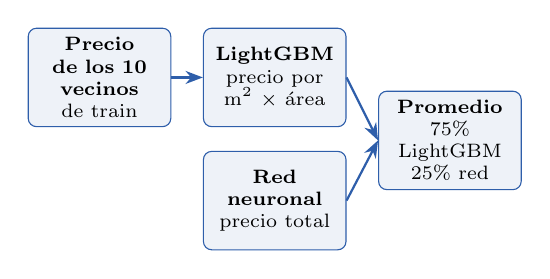
\begin{tikzpicture}[node distance=4mm]
        \node[pieza] (v) {\textbf{Precio de los 10 vecinos}\\ de train};
        \node[pieza, right=of v] (l) {\textbf{LightGBM}\\ precio por m\textsuperscript{2} $\times$ \'area};
        \node[pieza, below=3mm of l] (n) {\textbf{Red neuronal}\\ precio total};
        \node[pieza, right=of l, yshift=-8mm] (r) {\textbf{Promedio}\\ \PesoLgbm{} LightGBM\\ \PesoRed{} red};
        \draw[flecha] (v) -- (l);
        \draw[flecha] (l.east) -- (r.west);
        \draw[flecha] (n.east) -- (r.west);
      \end{tikzpicture}
    \end{column}
    \begin{column}{0.49\textwidth}
      \begin{block}{Lo que muestra este deck}
        \small
        \begin{enumerate}\setlength{\itemsep}{3pt}
          \item \textbf{La ubicaci\'on manda:} lo que m\'as predice el precio es cu\'anto valen las viviendas de al lado, y despu\'es el tama\~no.
          \item \textbf{El error real es mayor del que promete la validaci\'on cruzada,} y el modelo subestima las viviendas caras y sobrestima las baratas.
          \item \textbf{Sirve para comprar, pero no al precio que predice:} hay que ofrecer \MargenRegla{} menos para que solo 1 de cada 10 compras se pague de m\'as.
        \end{enumerate}
      \end{block}
    \end{column}
  \end{columns}
\end{frame}

% ============================================================
\section{Datos}
% ============================================================

\begin{frame}{Chapinero no es la Bogot\'a promedio}
  \begin{columns}[c, onlytextwidth]
    \begin{column}{0.64\textwidth}
      \centering
      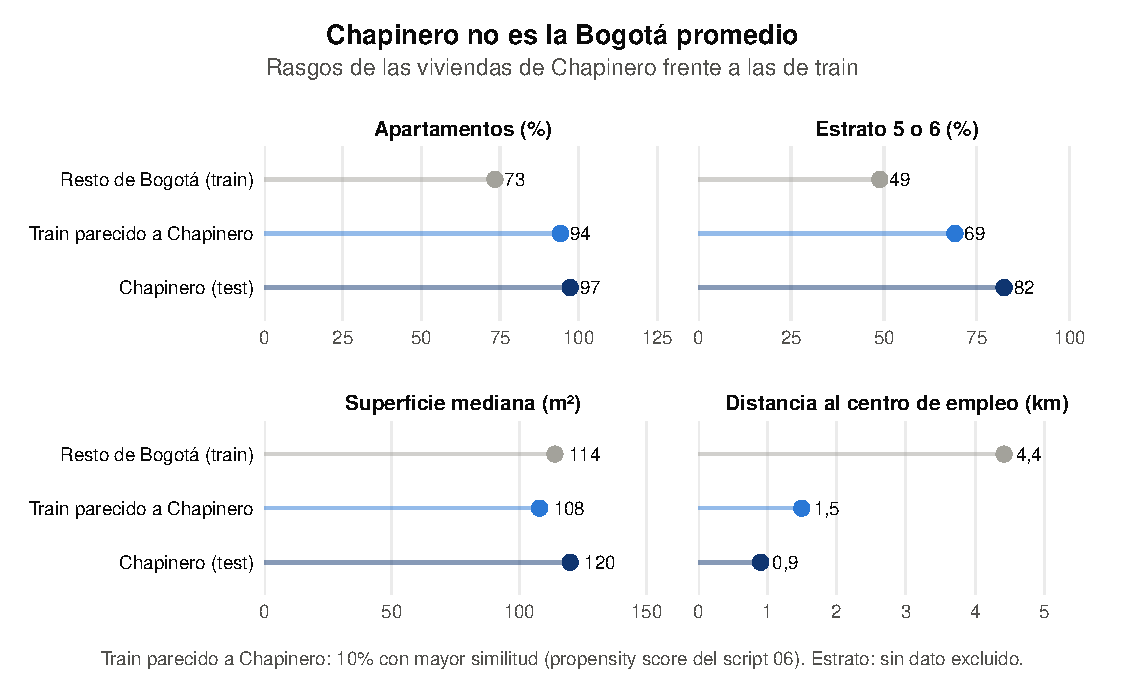
\includegraphics[width=\linewidth, height=0.82\textheight, keepaspectratio]{best_chapinero_distinto}
    \end{column}
    \begin{column}{0.33\textwidth}
      \footnotesize
      \begin{itemize}
        \item \textbf{Train:} \NTrain{} anuncios de Bogot\'a con precio. \textbf{Test:} \NTest{} anuncios de Chapinero, sin precio.
        \item Chapinero es casi todo apartamentos, de estrato 5 y 6, a menos de 1 km del centro de empleo.
        \item Las viviendas de train m\'as parecidas a Chapinero est\'an en las zonas vecinas.
      \end{itemize}
    \end{column}
  \end{columns}
\end{frame}

\begin{frame}{Probamos dos conjuntos de variables: 17 y 174}
  \vspace{1mm}
  \begin{columns}[T, onlytextwidth]
    \begin{column}{0.31\textwidth}
      \begin{block}{Base: 17 variables}
        \footnotesize
        Solo lo que trae la base de Kaggle.
        \begin{itemize}\setlength{\itemsep}{1pt}
          \item \textbf{Vivienda:} superficie, ba\~nos, ambientes, habitaciones, tipo, coordenadas y fecha.
          \item \textbf{Calidad del dato:} indicadores de superficie problem\'atica y de dato imputado.
        \end{itemize}
      \end{block}
    \end{column}
    \begin{column}{0.31\textwidth}
      \begin{block}{Completo: 174 variables}
        \footnotesize
        La base m\'as:
        \begin{itemize}\setlength{\itemsep}{1pt}
          \item \textbf{Entorno (OpenStreetMap y datos abiertos):} estrato de la manzana, distancia al centro de empleo, a TransMilenio, a v\'ias, parques, centros comerciales y universidades; zona verde, restaurantes y pendiente.
          \item \textbf{Texto del anuncio:} parqueaderos, piso y \NRaices{} palabras.
        \end{itemize}
      \end{block}
    \end{column}
    \begin{column}{0.33\textwidth}
      \begin{block}{Mejor modelo: 177 variables}
        \footnotesize
        El completo m\'as:
        \begin{itemize}\setlength{\itemsep}{1pt}
          \item \textbf{Precio de los vecinos:} mediana del precio y del precio por m\textsuperscript{2} de las 10 viviendas de train m\'as cercanas, y su distancia.
          \item \textbf{Precio por m\textsuperscript{2}} como variable a predecir, solo donde se conoce el \'area (\PctSuperficieReal{} de Chapinero). Donde no, el \'area se imput\'o con la mediana de su tipo de vivienda y el modelo predice el precio total.
        \end{itemize}
      \end{block}
    \end{column}
  \end{columns}
  \nota{Los datos faltantes se imputan con la mediana de su tipo de vivienda y se marcan con un indicador, para que el modelo distinga un dato imputado de uno real.}
\end{frame}

\begin{frame}{¿Qu\'e palabras del anuncio ayudan a predecir el precio?}
  \begin{columns}[c, onlytextwidth]
    \begin{column}{0.62\textwidth}
      \centering
      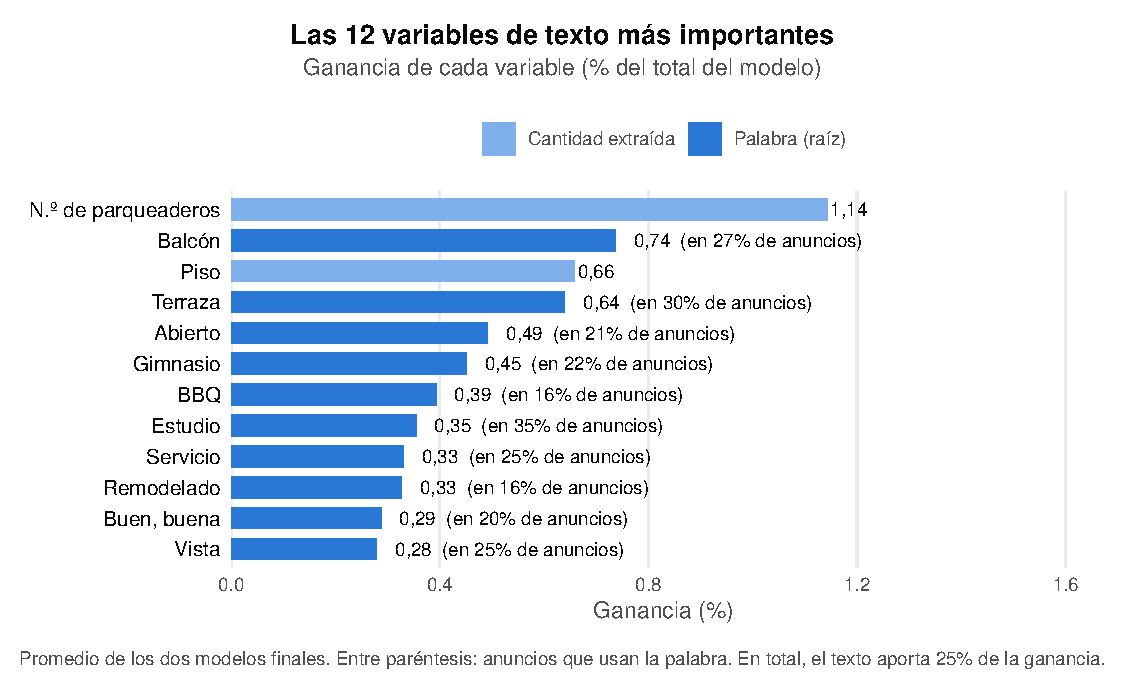
\includegraphics[width=\linewidth, height=0.82\textheight, keepaspectratio]{best_texto_importancia}
    \end{column}
    \begin{column}{0.35\textwidth}
      \footnotesize
      \begin{itemize}
        \item \textbf{Bolsa de palabras:} limpiamos la descripci\'on, reducimos cada palabra a su ra\'iz y marcamos 1 si el anuncio la usa.
        \item \textbf{Regla del 5\%:} solo entran las ra\'ices que aparecen en al menos el 5\% de los anuncios (\NRaices).
        \item \textbf{Qu\'e capta:} parqueaderos, balc\'on, terraza, gimnasio y BBQ son se\~nales de calidad que no est\'an en las variables de la base. En total, el texto aporta \GainTexto\% de la ganancia.
      \end{itemize}
    \end{column}
  \end{columns}
\end{frame}

% ============================================================
\section{Validaci\'on}
% ============================================================

\begin{frame}{Tres validaciones cruzadas: la aleatoria es demasiado optimista}
  \centering
  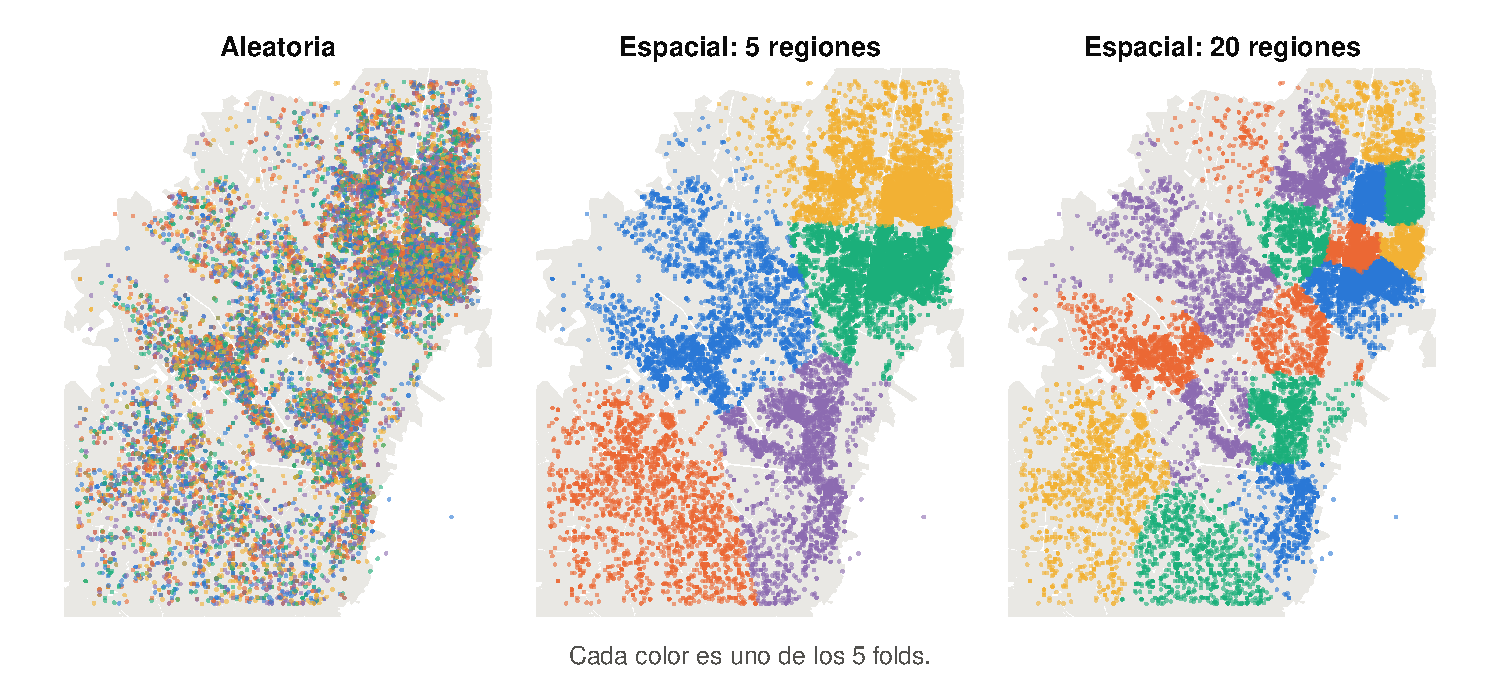
\includegraphics[width=\linewidth, height=0.6\textheight, keepaspectratio]{best_cv_esquemas}
  \vspace{-1mm}
  \begin{columns}[T, onlytextwidth]
    \begin{column}{0.31\textwidth}
      \scriptsize
      {\footnotesize\bfseries\color{azuloscuro}Promete \PrometeAleatoria\% menos error del real}\\[1mm]
      Al azar: cada vivienda tiene vecinas del mismo edificio en entrenamiento. M\'as f\'acil que Chapinero.
    \end{column}
    \begin{column}{0.31\textwidth}
      \scriptsize
      {\footnotesize\bfseries\color{azuloscuro}Promete \PrometeCinco\% m\'as error del real}\\[1mm]
      Cada fold es una regi\'on grande, muy lejos de lo que se entrena. M\'as dif\'icil que Chapinero.
    \end{column}
    \begin{column}{0.31\textwidth}
      \scriptsize
      {\footnotesize\bfseries\color{accent}Promete \PrometeVeinte\% menos error del real: la elegida}\\[1mm]
      20 zonas del tama\~no de un barrio, en 5 folds. La m\'as parecida a predecir Chapinero.
    \end{column}
  \end{columns}
\end{frame}

\begin{frame}{Ni la CV espacial nos dice el error en Chapinero: creamos pseudo-Chapineros}
  \begin{columns}[c, onlytextwidth]
    \begin{column}{0.42\textwidth}
      \centering
      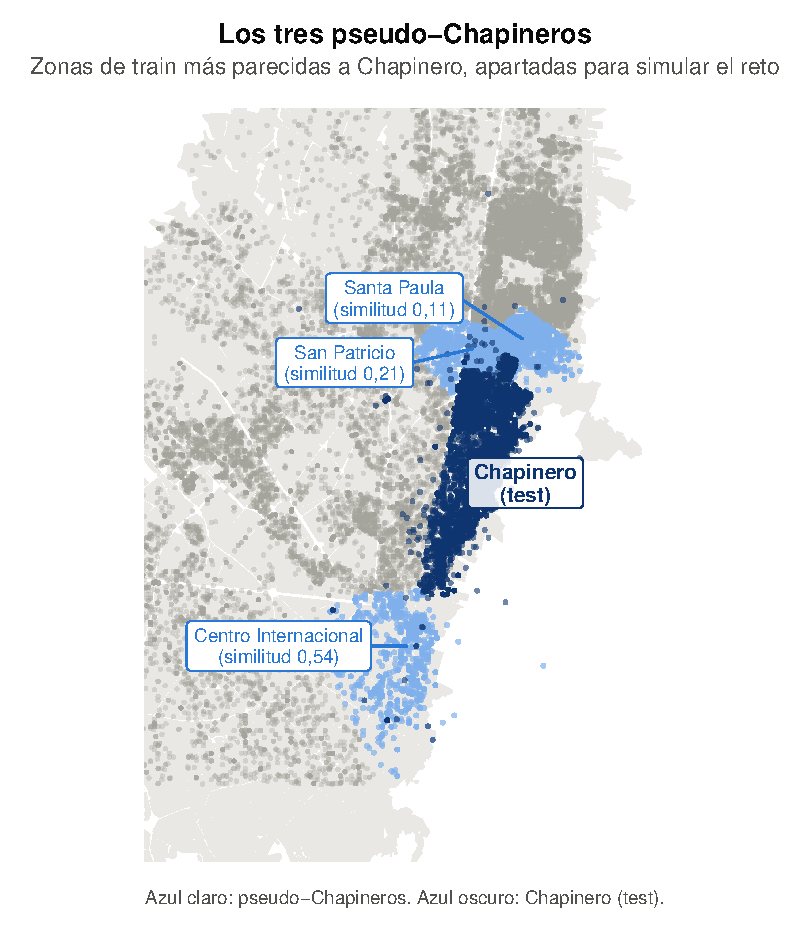
\includegraphics[width=\linewidth, height=0.86\textheight, keepaspectratio]{best_pseudo_chapinero_mapa}
    \end{column}
    \begin{column}{0.55\textwidth}
      \small
      Sin precios en Chapinero no podemos medir qu\'e validaci\'on anticipa su error. Lo simulamos dentro de train:
      \begin{enumerate}\setlength{\itemsep}{3pt}
        \item Elegimos las 3 zonas de train \textbf{m\'as parecidas a Chapinero} (regresi\'on log\'istica con las caracter\'isticas de la vivienda y del entorno).
        \item Las apartamos y medimos el \textbf{error real} en ellas.
        \item Lo comparamos con el error que \textbf{promet\'ia cada validaci\'on}.
      \end{enumerate}
      \vspace{2mm}
      De aqu\'i salen los porcentajes de la slide anterior.
    \end{column}
  \end{columns}
  \nota{Promedio de 3 zonas y 2 modelos (Random Forest y regresi\'on lineal).}
\end{frame}

% ============================================================
\section{El modelo}
% ============================================================

\begin{frame}{El modelo final, paso a paso}
  \centering
  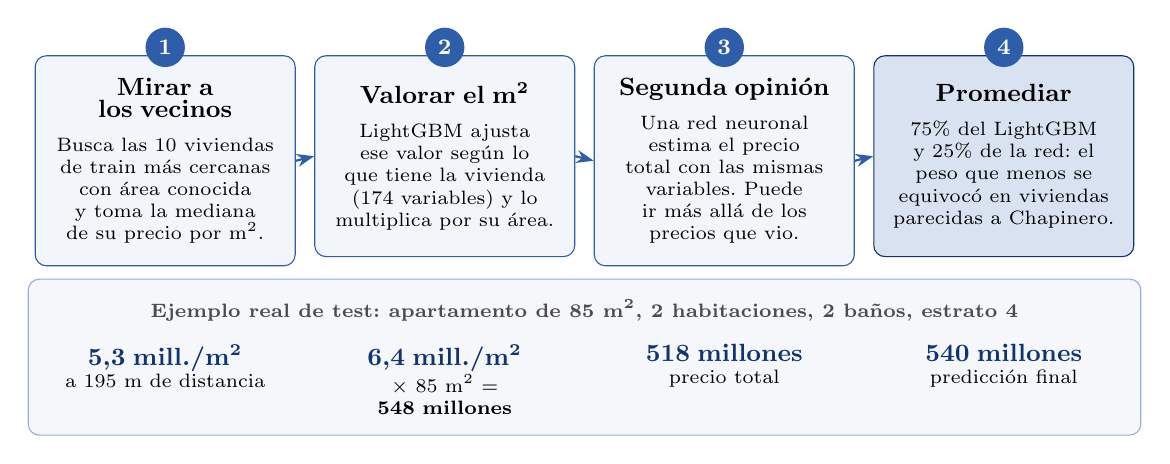
\begin{tikzpicture}[x=1cm, y=1cm]
    \foreach \i/\x in {1/0, 2/3.55, 3/7.1, 4/10.65} {
      \coordinate (p\i) at (\x, 0);
    }
    \node[paso] (a) at (p1) {{\small\bfseries Mirar a los vecinos}\\[1.5mm]
      Busca las 10 viviendas de train m\'as cercanas con \'area conocida y toma la mediana de su precio por m\textsuperscript{2}.};
    \node[paso] (b) at (p2) {{\small\bfseries Valorar el m\textsuperscript{2}}\\[1.5mm]
      LightGBM ajusta ese valor seg\'un lo que tiene la vivienda (174 variables) y lo multiplica por su \'area.};
    \node[paso] (c) at (p3) {{\small\bfseries Segunda opini\'on}\\[1.5mm]
      Una red neuronal estima el precio total con las mismas variables. Puede ir m\'as all\'a de los precios que vio.};
    \node[paso, fill=accent!18, draw=azuloscuro] (d) at (p4) {{\small\bfseries Promediar}\\[1.5mm]
      \PesoLgbm{} del LightGBM y \PesoRed{} de la red: el peso que menos se equivoc\'o en viviendas parecidas a Chapinero.};
    \foreach \u/\v in {a/b, b/c, c/d} {
      \draw[flecha] (\u.east) -- (\v.west);
    }
    \foreach \n/\k in {a/1, b/2, c/3, d/4} {
      \node[numero, yshift=1mm] at (\n.north) {\k};
    }
    % Ejemplo, en una caja aparte debajo de los pasos.
    \foreach \n/\x in {ea/0, eb/3.55, ec/7.1, ed/10.65} {
      \coordinate (\n) at (\x, -3.55);
    }
    \node[valor] (va) at (ea) {\valorpaso{\EjVecinosMdos{} mill./m\textsuperscript{2}}\\ a \EjVecinosDist{} m de distancia};
    \node[valor] (vb) at (eb) {\valorpaso{\EjLgbmMdos{} mill./m\textsuperscript{2}}\\ $\times$ \EjSuperficie{} m\textsuperscript{2} = \textbf{\EjLgbm{} millones}};
    \node[valor] (vc) at (ec) {\valorpaso{\EjRed{} millones}\\ precio total};
    \node[valor] (vd) at (ed) {\valorpaso{\EjFinal{} millones}\\ predicci\'on final};
    \node[anchor=south, font=\scriptsize\bfseries, color=black!70] (te) at ($(va.north)!0.5!(vd.north) + (0, 0.05)$)
      {Ejemplo real de test: apartamento de \EjSuperficie{} m\textsuperscript{2}, \EjHabitaciones{} habitaciones, \EjBanos{} ba\~nos, estrato \EjEstrato};
    \begin{scope}[on background layer]
      \node[draw=accent!50, fill=accent!5, rounded corners=4pt, inner sep=4pt,
        fit=(te) (va) (vb) (vc) (vd)] {};
    \end{scope}
  \end{tikzpicture}

  \vspace{2mm}
  {\footnotesize \textbf{Por qu\'e funciona:} los vecinos aportan la \alert{ubicaci\'on}, el m\textsuperscript{2} permite \alert{trasladar} ese valor a viviendas de otro tama\~no y la red corrige que los \'arboles \alert{no extrapolan}.\par}
  \nota{Si el anuncio no trae el \'area (\PctSuperficieImputada{} de Chapinero), el paso 2 predice directamente el precio total.}
\end{frame}

\begin{frame}{Del MAE de \MAEBase{} millones al de \MAEKaggle}
  \begin{columns}[c, onlytextwidth]
    \begin{column}{0.62\textwidth}
      \centering
      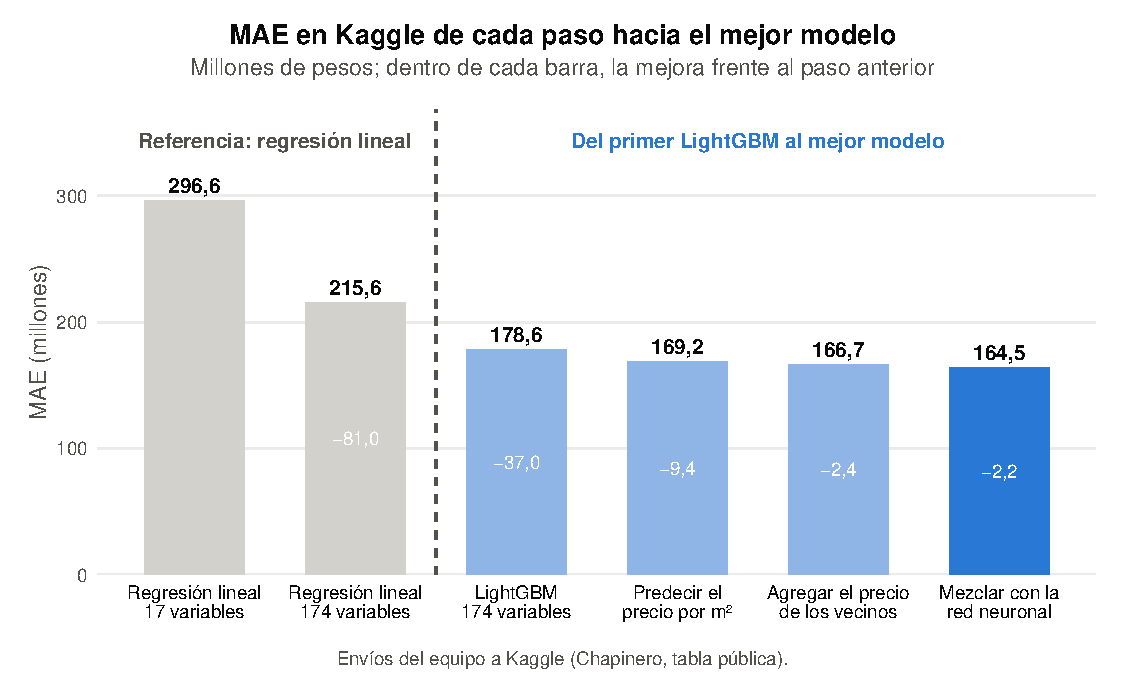
\includegraphics[width=\linewidth, height=0.82\textheight, keepaspectratio]{best_cascada_kaggle}
    \end{column}
    \begin{column}{0.35\textwidth}
      \footnotesize
      \begin{itemize}\setlength{\itemsep}{2pt}
        \item \textbf{Referencia (gris):} la misma regresi\'on lineal con 17 y con 174 variables. La diferencia (\MejoraLMTexto{} millones) es lo que aportan las variables de entorno y de texto.
        \item \textbf{LightGBM} con esas 174 variables baja otros 37: capta relaciones no lineales e interacciones.
        \item \textbf{Precio por m\textsuperscript{2} y vecinos} atacan el problema de Chapinero: trasladar el valor de la ubicaci\'on.
        \item \textbf{La red neuronal} baja \MejoraRed{} m\'as: los \'arboles no predicen fuera de los precios que vieron; la red s\'i, y al promediar se corrigen los extremos.
      \end{itemize}
    \end{column}
  \end{columns}
\end{frame}

\begin{frame}{Entrenamiento y elecci\'on de hiperpar\'ametros}
  \vspace{2mm}
  \centering
  {\footnotesize
  \begin{tabular}{>{\raggedright\arraybackslash}p{0.2\textwidth}>{\raggedright\arraybackslash}p{0.68\textwidth}}
    \toprule
    Decisi\'on & Qu\'e hicimos \\
    \midrule
    Algoritmo & LightGBM (boosting). \\
    P\'erdida & MAE. \\
    Hiperpar\'ametros & B\'usqueda aleatoria de \NEnsayos{} combinaciones con la validaci\'on de 20 regiones. Ganadora: tasa de aprendizaje \TasaAprendizaje, \Hojas{} hojas, profundidad \Profundidad, m\'inimo \MinHoja{} viviendas por hoja, \Rondas{} rondas (parada temprana). \\
    Variable a predecir & Precio por m\textsuperscript{2} $\times$ \'area donde el \'area se conoce; precio total donde se imput\'o. \\
    Vecinos & 10 vecinos de train; en la validaci\'on cruzada, solo de los datos de entrenamiento. \\
    Red neuronal & 3 capas ocultas (256, 128 y 64 neuronas); en cada paso apaga al azar el 30\% de las neuronas (\emph{dropout}) para no sobreajustar. \\
    Mezcla & \PesoLgbm{} LightGBM + \PesoRed{} red: el peso que minimiza el error en las viviendas parecidas a Chapinero. \\
    \bottomrule
  \end{tabular}}
  \nota{Todos los modelos se eval\'uan con las mismas particiones de la validaci\'on cruzada, para que sus errores sean comparables.}
\end{frame}

\begin{frame}{¿Qu\'e mira el modelo? Primero la ubicaci\'on, luego el tama\~no}
  \begin{columns}[c, onlytextwidth]
    \begin{column}{0.75\textwidth}
      \centering
      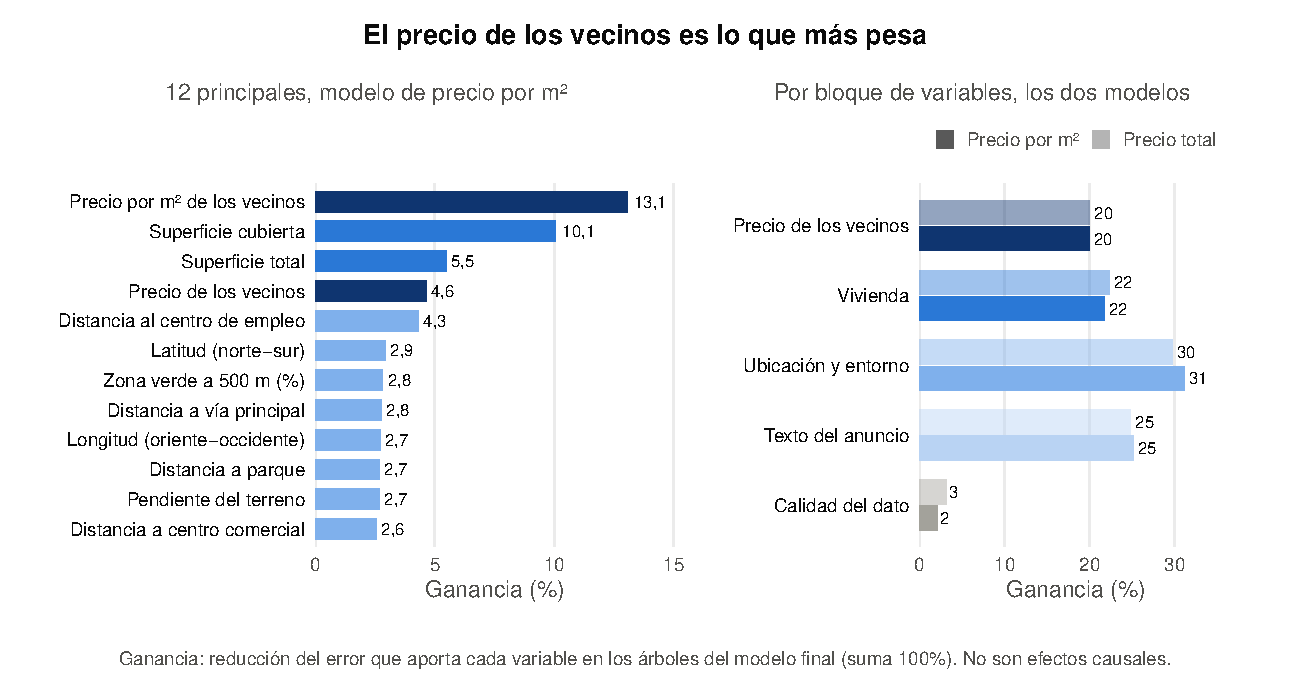
\includegraphics[width=\linewidth, height=0.88\textheight, keepaspectratio]{best_importancia}
    \end{column}
    \begin{column}{0.23\textwidth}
      \footnotesize
      \begin{itemize}
        \item El precio por m\textsuperscript{2} de los vecinos es la variable principal: resume cu\'anto vale la zona.
        \item \textbf{Por bloques, la ubicaci\'on suma \GainUbicacion\%} de la ganancia (entorno y vecinos), la vivienda \GainVivienda\% y el texto \GainTexto\%.
        \item No son efectos causales.
      \end{itemize}
    \end{column}
  \end{columns}
\end{frame}

\begin{frame}{La validaci\'on cruzada promete menos error del que tuvimos en Chapinero}
  \begin{columns}[c, totalwidth=0.94\textwidth]
    \begin{column}{0.52\textwidth}
      \centering
      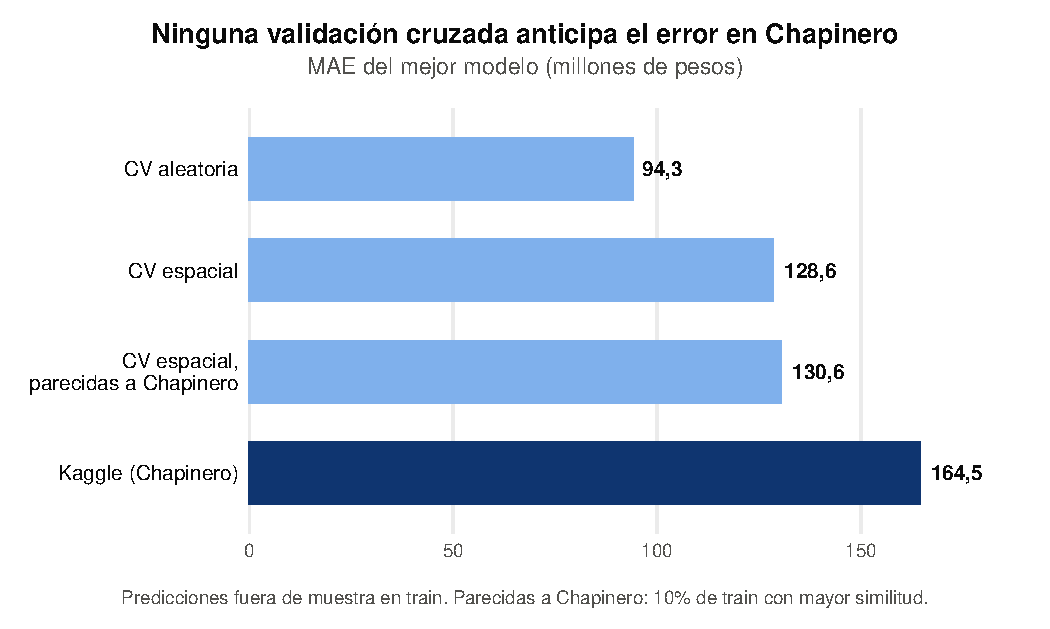
\includegraphics[width=\linewidth, height=0.8\textheight, keepaspectratio]{best_cv_frente_kaggle}
    \end{column}
    \begin{column}{0.44\textwidth}
      \footnotesize
      \begin{itemize}
        \item \textbf{Nivel:} en Kaggle el error (\MAEKaggle) fue mayor que en cualquier validaci\'on. Chapinero fue m\'as dif\'icil de lo que se puede simular con train.
        \item \textbf{Orden:} al agregar los vecinos, las validaciones no coincidieron. Kaggle le dio la raz\'on a la aleatoria.
      \end{itemize}
      \vspace{1mm}
      \centering
      {\scriptsize\setlength{\tabcolsep}{4pt}
      \begin{tabular}{lccc}
        \toprule
        MAE (millones) & CV espacial & CV aleatoria & Kaggle \\
        \midrule
        Sin vecinos & \CVEspSinVec & \CVAleSinVec & \KaggleSinVec \\
        Con vecinos & \CVEspConVec & \CVAleConVec & \KaggleConVec \\
        \midrule
        ¿Mejora? & \textbf{No} & \textcolor{accent}{\textbf{S\'i}} & \textcolor{accent}{\textbf{S\'i}} \\
        \bottomrule
      \end{tabular}}
    \end{column}
  \end{columns}
\end{frame}

\begin{frame}{El modelo sobrestima las viviendas baratas y subestima las caras}
  \begin{columns}[c, onlytextwidth]
    \begin{column}{0.64\textwidth}
      \centering
      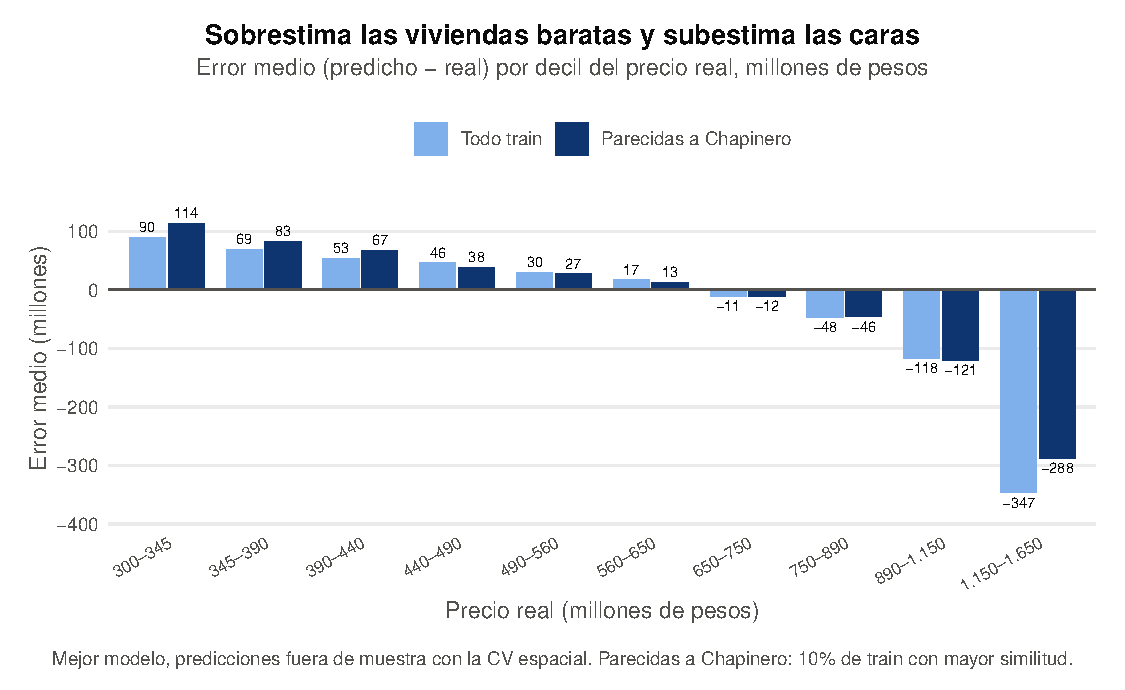
\includegraphics[width=\linewidth, height=0.82\textheight, keepaspectratio]{best_sesgo_deciles}
    \end{column}
    \begin{column}{0.33\textwidth}
      \footnotesize
      \begin{itemize}
        \item \textbf{Regresi\'on a la media:} en el 10\% m\'as barato sobrestima \SesgoBaratas{} millones en promedio; en el 10\% m\'as caro subestima \SesgoCaras.
        \item En las viviendas parecidas a Chapinero (azul oscuro) el patr\'on es el mismo, y en promedio se queda corto (\SesgoSimilares{} millones).
        \item Ese promedio esconde que en muchas viviendas el modelo predice de m\'as, y cada una de esas compras se pagar\'ia por encima de su precio.
      \end{itemize}
    \end{column}
  \end{columns}
\end{frame}

% ============================================================
\section{Negocio}
% ============================================================

\begin{frame}{Sobrestimar y subestimar no cuestan lo mismo}
  \begin{columns}[c, onlytextwidth]
    \begin{column}{0.62\textwidth}
      \centering
      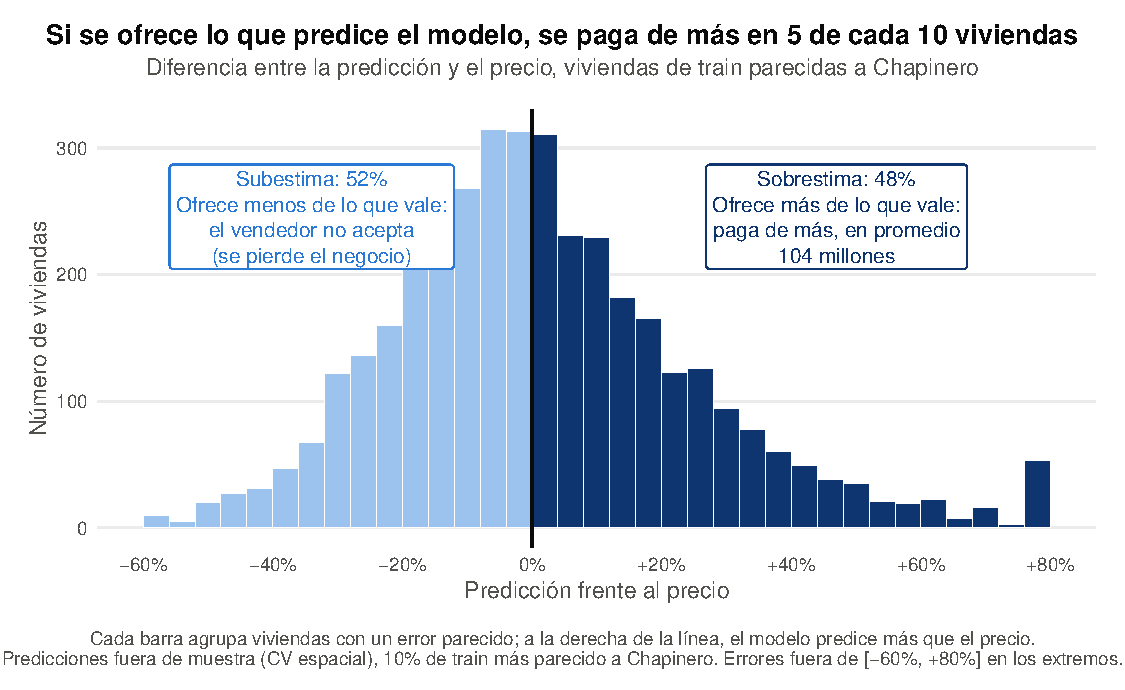
\includegraphics[width=\linewidth, height=0.82\textheight, keepaspectratio]{negocio_errores}
    \end{column}
    \begin{column}{0.35\textwidth}
      \footnotesize
      \begin{itemize}
        \item \textbf{Subestima (\PctSub):} si la empresa ofrece la predicci\'on, el vendedor no acepta. Se pierde un negocio, no dinero.
        \item \textbf{Sobrestima (\PctSobre):} la oferta supera el precio y la empresa paga de m\'as, en promedio \SobrepagoMedio{} millones por vivienda.
        \item El MAE cuenta igual los dos errores; para el negocio solo el segundo destruye capital.
      \end{itemize}
    \end{column}
  \end{columns}
\end{frame}

\begin{frame}{Regla de compra: ofrecer \MargenRegla{} menos de lo que predice el modelo}
  \begin{columns}[c, onlytextwidth]
    \begin{column}{0.62\textwidth}
      \centering
      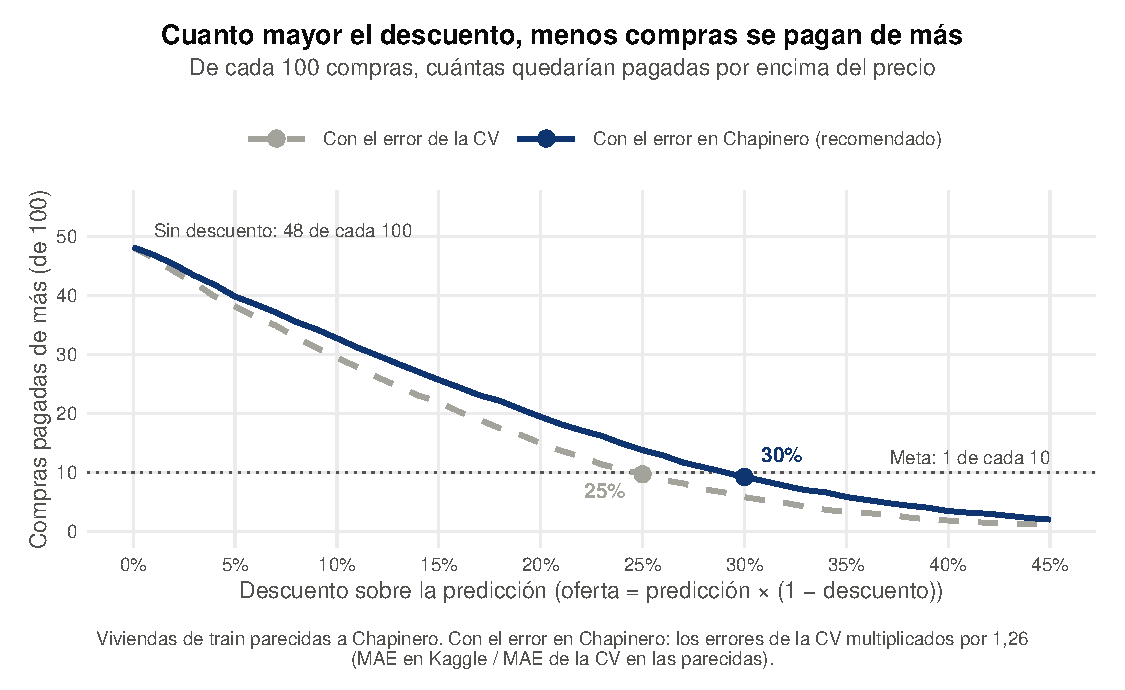
\includegraphics[width=\linewidth, height=0.82\textheight, keepaspectratio]{negocio_margen}
    \end{column}
    \begin{column}{0.35\textwidth}
      \footnotesize
      \begin{itemize}
        \item Sin descuento, \RiesgoSinMargen{} de las compras se pagan de m\'as.
        \item \textbf{Meta:} la regla supone que solo 1 de cada 10 compras puede quedar pagada por encima del precio. La empresa puede ajustarla seg\'un su tolerancia al riesgo y leer en la curva el descuento que le corresponde.
        \item \textbf{Error en Chapinero:} fue \FactorKaggle{} veces el de la validaci\'on cruzada. Con el error de la CV bastar\'ia \MargenCV; con el de Chapinero hace falta \MargenRegla.
        \item \textbf{Trade-off:} m\'as descuento, menos riesgo, pero ofertas m\'as bajas (la t\'ipica queda \OfertaTipica{} bajo el precio) y menos vendedores que acepten.
      \end{itemize}
    \end{column}
  \end{columns}
\end{frame}

\begin{frame}{D\'onde no confiar en el modelo: las casas}
  \begin{columns}[c, onlytextwidth]
    \begin{column}{0.62\textwidth}
      \centering
      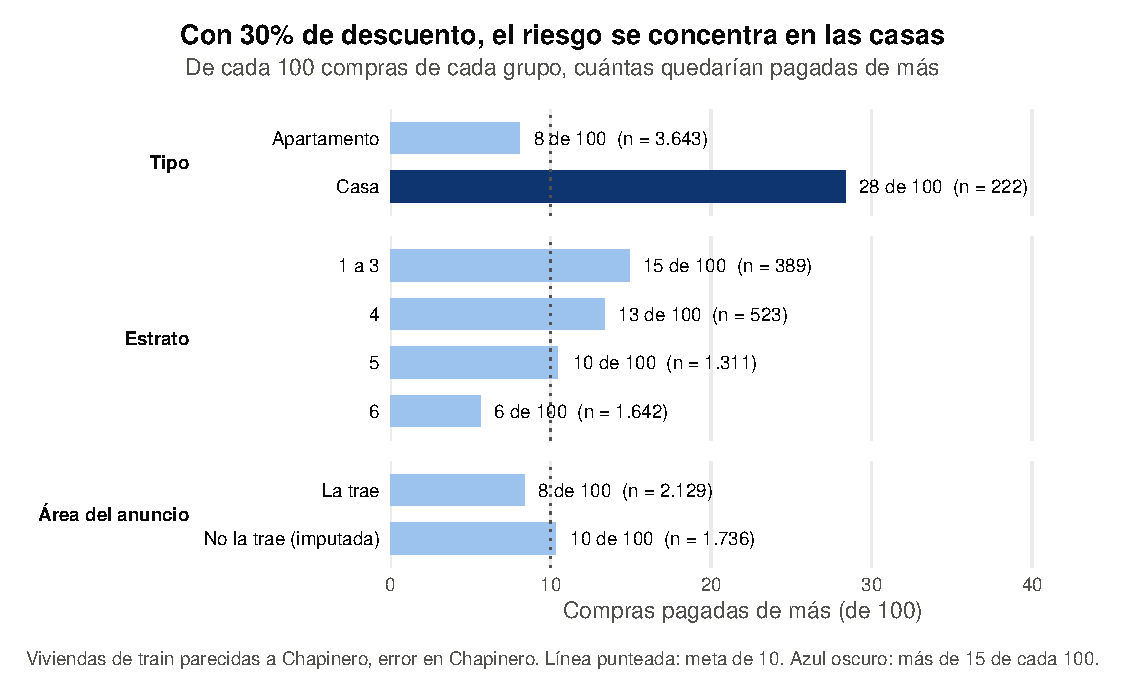
\includegraphics[width=\linewidth, height=0.84\textheight, keepaspectratio]{negocio_donde_confiar}
    \end{column}
    \begin{column}{0.35\textwidth}
      \footnotesize
      \begin{itemize}
        \item Con el descuento de \MargenRegla, agrupamos las viviendas con lo que se sabe \textbf{antes} de comprar.
        \item \textbf{Casas:} \RiesgoCasa{} de las compras se pagar\'ian de m\'as, casi el triple de la meta. Los \textbf{estratos 1 a 3} tambi\'en la superan (\RiesgoEstBajo).
        \item \textbf{Estrato 6}, lo t\'ipico de Chapinero: \RiesgoEstSeis.
        \item Que el anuncio traiga o no el \'area casi no cambia el riesgo (\RiesgoReal{} frente a \RiesgoImputada).
      \end{itemize}
    \end{column}
  \end{columns}
\end{frame}

\begin{frame}{¿Podemos confiar en este modelo para comprar? S\'i, con condiciones}
  \vspace{3mm}
  \begin{columns}[T, onlytextwidth]
    \begin{column}{0.48\textwidth}
      \begin{alertblock}{1. Predice bien el valor de la zona}
        \footnotesize La ubicaci\'on (entorno y precio de los vecinos) explica \GainUbicacion\% de lo que usa el modelo, y el tama\~no hace el resto.
      \end{alertblock}
      \begin{alertblock}{2. La validaci\'on cruzada es optimista}
        \footnotesize En Chapinero el error fue \FactorKaggle{} veces el que promet\'ia la validaci\'on cruzada. La regla de compra ya usa ese error mayor.
      \end{alertblock}
    \end{column}
    \begin{column}{0.48\textwidth}
      \begin{alertblock}{3. Comprar solo con descuento}
        \footnotesize Ofrecer la predicci\'on menos \MargenRegla: las compras pagadas de m\'as bajan de \RiesgoSinMargen{} a \RiesgoRegla. El modelo sirve para filtrar oportunidades, no para fijar el precio.
      \end{alertblock}
      \begin{alertblock}{4. Verificar donde falla}
        \footnotesize En casas y estratos bajos el riesgo sigue alto: aval\'uo o visita antes de ofertar.
      \end{alertblock}
    \end{column}
  \end{columns}
  \nota{Limitaciones: los precios son de oferta en el anuncio, no de cierre; hay anuncios repetidos; y si en Chapinero hay viviendas m\'as caras que en train, ah\'i el modelo subestima.}
\end{frame}

\begin{frame}{Oportunidades de mejora}
  \vspace{2mm}
  \begin{columns}[T, onlytextwidth]
    \begin{column}{0.48\textwidth}
      \begin{block}{M\'as y mejores datos}
        \footnotesize
        \begin{itemize}\setlength{\itemsep}{2pt}
          \item \textbf{Precios de cierre} en lugar de precios de oferta del anuncio.
          \item \textbf{Aprender de Chapinero:} agregar al entrenamiento las viviendas que la empresa compre y venda all\'i.
          \item \textbf{\'Area real de todas las viviendas} (catastro o visita): hoy falta en el \PctSuperficieImputada{} de Chapinero, y sin ella no se puede usar el precio por m\textsuperscript{2}.
        \end{itemize}
      \end{block}
    \end{column}
    \begin{column}{0.48\textwidth}
      \begin{block}{Mejor modelo y mejor validaci\'on}
        \footnotesize
        \begin{itemize}\setlength{\itemsep}{2pt}
          \item \textbf{Un precio conservador para cada vivienda:} predecir un percentil bajo del precio (p\'erdida por cuantiles) en lugar de aplicar el mismo descuento a todas.
          \item \textbf{Un modelo aparte para casas,} donde el error es mayor.
          \item \textbf{Una validaci\'on que respete la distancia real a los vecinos:} la CV espacial los aleja m\'as que en Chapinero y por eso juzg\'o mal esa variable.
        \end{itemize}
      \end{block}
    \end{column}
  \end{columns}
\end{frame}

% ============================================================
\appendix

\begin{frame}[standout]
  ¡Gracias!
\end{frame}

\end{document}
